\documentclass{article}

\usepackage{Mathematics}
\pdftitle{Mathematics 3A}

% === TITLE ===
\title{\textbf{Mathematics 3A \\ HSLU, Semester 3}}
\author{Matteo Frongillo}
\date{}

% === TEXT ===
\begin{document}

\maketitle
\tableofcontents
\pagebreak

\part{Just stuff I have to explain, wait few days}
Let $\pi$ denote the plane:
\[s_y\in \pi, s_y\in\pi, s_z\in\pi\]
\[\pi: ax+by+cz+d=0\qquad \]

For $S_x\in\pi \Longrightarrow 1a+0b+0c+d = 0$, hence\\
$a+d=0$

For $S_y\in\pi \Longrightarrow 0a+2b+0c+d=0$, hence\\
$2b+d=0$

for $S_z\in\pi \Longrightarrow 0a+0b+3c+d=0$, hence\\
$3c+d=0$

\[
\begin{cases}
    a+d=0\\
    2b+d=0\\
    3c+d=0
\end{cases}
\Longrightarrow
\begin{cases}
    a=-d\\
    2b=-d\\
    3c=-d
\end{cases}
\]

Case 1:
\[d=0 \Longrightarrow a=0, b=0, c=0 \Longrightarrow \pi: 0=0 \Longrightarrow \text{NOT a plane!}\]

Case 2:
\[d\neq0 \Longrightarrow \pi:\frac{ax+by+cz+d}{d} = 0 \Longrightarrow \frac{a}{d}x + \frac{b}{d}y + \frac{c}{d}z + 1 = 0\]

Hence:
\[
\begin{cases}
    a=-d\\
    2b=-d\\
    3c=-d
\end{cases}
\Longrightarrow
\begin{cases}
    \frac{a}{d} = -1\\
    \frac{b}{d} = -\frac{1}{2}\\
    \frac{c}{d} = -\frac{1}{3}
\end{cases}
\]

Which leads to:
\[\pi: -x-\frac{1}{2}y-\frac{1}{3}z + 1 = 0\]

\rem{the equation of a plane is defined up to a multiplication by a real number different from 0}

e.g.: the same planed is shared between those 3 equations\\
ex 1)
\[z=0 \Longleftrightarrow 5z=0 \Longleftrightarrow -10z=0\]

ex 2)
\[-x-\frac{1}{2}y-\frac{1}{3}z + 1 = 0 \Longleftrightarrow 6x+3y+2z+6=0\]


\newpage
\section{Functions in two variables $x$ and $y$}
Let us take $\pi:x^2-y^2=0$ as example.

The plot would look like this:

\begin{center}
    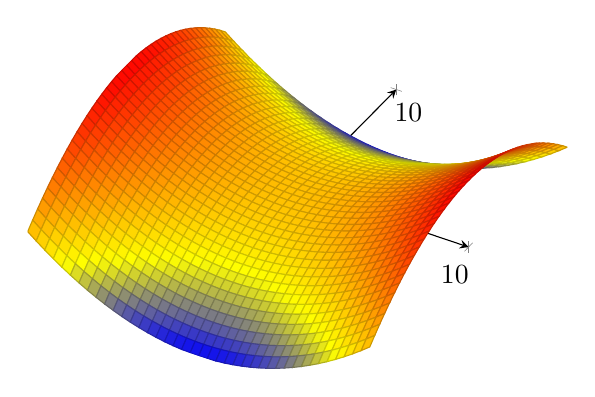
\begin{tikzpicture}
      \begin{axis}[view={30}{60}, axis lines=middle, domain=-10:10, y domain=-10:10, samples=41]
        \addplot3[surf] {x^2 - y^2};
      \end{axis}
    \end{tikzpicture}
\end{center}

\subsection{Spheres}

\section{Linear functions of two variables}
We say that $z$ is a \textit{linear function} of $x$ and $y$, if there are
constant $a,b$ and $d$ such that:
\figbox{$\dm z = ax + by + d$}

holds. Alternatively: if there are constant $A,B,C,D$, with $C \neq 0$, such that:
\figbox{$\dm Az + Bx + Cy + D = 0$}

holds. Since $C \neq 0$, we can rearrange this equation into:
\figbox{$\dm z = -\frac{Ax}{C} - \frac{By}{C} - \frac{D}{C}$}

\newpage
\section{Contour lines}
\[
\begin{cases}
    z = f(x,y)\\
    z = k \qquad k\in\mathbb{R}
\end{cases}
\]

$z=k$ represents all the possible horizontal planes

Ex:
\[
\begin{cases}
    z = x^2 - y^2\\
    z = k
\end{cases} \Longrightarrow
\begin{cases}
    k = x^2 - y^2\\
    z = k
\end{cases}
\]

\begin{center}
    \pgfplotsset{compat=1.18}
    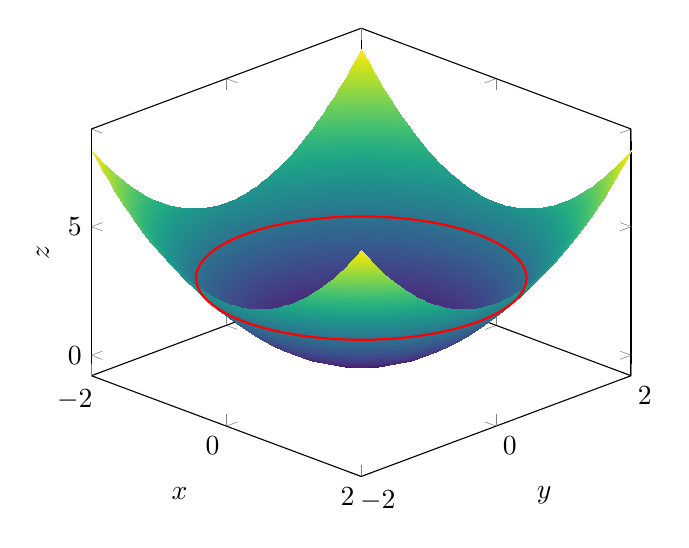
\begin{tikzpicture}
        \begin{axis}[
            view={45}{30},
            xlabel={$x$},
            ylabel={$y$},
            zlabel={$z$},
            domain=-2:2,
            y domain=-2:2,
            samples=50,
            colormap/viridis
        ]
            % Surface z = x^2 + y^2
            \addplot3[surf, shader=interp] {x^2 + y^2};

            % Contour circle at z = 3, i.e. x^2 + y^2 = 3
            \addplot3[
            domain=0:360,
            samples=100,
            thick,
            color=red
            ] (
            {sqrt(3)*cos(x)},
            {sqrt(3)*sin(x)},
            {3}
            );
        \end{axis}
    \end{tikzpicture}
\end{center}

All the planes with equation $z=k$ are parallel to the coordinate planes $z=0$.

When $z=k=0$, the circle is reduced to a point, the origin.

When $k<0$, the equation $x^2+y^2=k$ has no solution in $\mathbb{R}$.

When $k>0$, the equation $x^2+y^2=k$ represents a circle with radius $\sqrt{k}$ centered at the origin.

\section{Cylinders}
A cylinder is a surface generated by all the lines parallel to a given line $d$ and passing through a given curve $\mathcal{C}$.

% Add plot

\subsection{Property}
Whenever you have a polynomial equation of degree at least 2 with a missing variable,
then you have a cylinder (up to few exceptions).

Ex:
\[ z = y^2 \Longrightarrow y^2 - z = 0 \]
This is a cylinder with generatrix parallel to the $x$ axis and directrix the
parabola $y^2 - z = 0$ in the $yz$ plane.

\begin{center}
    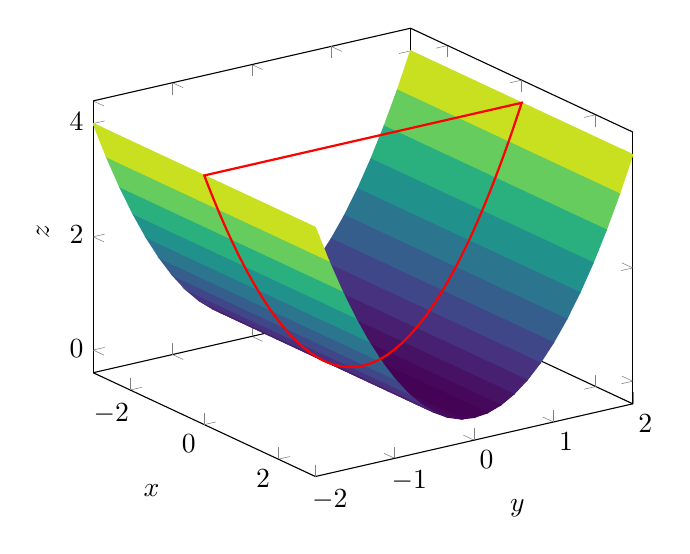
\begin{tikzpicture}
      \begin{axis}[
        view={55}{25},
        xlabel={$x$},
        ylabel={$y$},
        zlabel={$z$},
        domain=-3:3,
        y domain=-2:2,
        samples=25,
        samples y=25,
        shader=flat,
        colormap/viridis
      ]
        % Parabolic cylinder: z = y^2 (independent of x)
        \addplot3[surf] {y^2};
    
        % Directrix in the yz-plane (x = 0): z = y^2
        \addplot3[
          domain=-2:2,
          samples=200,
          thick,
          color=red
        ] ({0},{x},{x^2});
      \end{axis}
    \end{tikzpicture}
\end{center}

\newpage
\part{Partial derivatives}
For a multivariable function $f(x,y,...)$, the partial derivative to
one variable measures the instantaneous rate of change of $f$ when
that variable changes and the others are held constant:

\figbox{$\dm \frac{\partial z}{\partial x} = f_x(x,y)$}

If $z$ is a function of $x$ and $y$, we define:

The rate of change of $z$ with respect to $x$, with $y$ fixed, at the
point ($x,y$)=($a,b$) as
\figbox{$\dm \frac{\partial z}{\partial x} \big|_{(x,y)=(a,b)} = \lim_{h\to0}\frac{Z\big|_{(x,y)=(a+h,b)} - Z \big|_{(x,y)=(a,b)}}{h}$}

The rate of change of $z$ with respect to $y$, with $x$ fixed, at the
point $(x,y)=(a,b)$ as
\figbox{$\dm \frac{\partial z}{\partial x} \big|_{(x,y)=(a,b)} = \lim_{h\to0}\frac{Z\big|_{(x,y)=(a,b+h)} - Z \big|_{(x,y)=(a,b)}}{h}$}

For the lectures, we will be using the formula with 2-steps difference ($\Delta z_a = (a+h,b)-(a-h,b)$):
\figbox{$\dm \frac{\partial z}{\partial x} \big|_{(x,y)=(a,b)} = \frac{Z\big|_{(x,y)=(a+h,b)} - Z \big|_{(x,y)=(a-h,b)}}{2h}$\\\\
        $\dm \frac{\partial z}{\partial y} \big|_{(x,y)=(a,b)} = \frac{Z\big|_{(x,y)=(a,b+h)} - Z \big|_{(x,y)=(a,b-h)}}{2h}$}

\section{Local linearization}
\subsection{Tangent plane of a function at point P}
Let $f(x,y)$ be our function and $P(a,b)$ a point, $P \in f$:
\figbox{$\dm f(x,y) \approx f(a,b) + \frac{\partial}{\partial x} f(a,b)(x-a) + \frac{\partial}{\partial y} f(a,b)(y-b)$}

\section{Gradient}
The gradient of a function $z=f(x,y)$ is defined by:
\figbox{$\dm \text{grad } f = \nabla f = f_x\overrightarrow{e_x} + f_y\overrightarrow{e_y} = \binom{f_x}{f_y}$\\\\
        where $\dm f_x = \frac{\partial f}{\partial x}$ and $\dm f_y = \frac{\partial f}{\partial y}$}


\newpage
\subsection{Geometrical properties of the gradient vector $\nabla$ in the plane}
If $f$ is differentiable at the point $(a,b)$ and $\nabla f \neq \overrightarrow{0}$,
then the following holds:

$\mathbf{\nabla f(a,b)}$:
\begin{itemize}
    \item is perpendicular to the contour line of $f$ through $(a,b)$
    \item points in the direction of the maximum rate of change $f$
\end{itemize}

\textbf{The length $\mathbf{\left\lVert\nabla f(a,b)\right\rVert}$ of the gradient vector is}:
\begin{itemize}
    \item the maximum rate of change $f$ at this point
    \item large when the contour lines are close together
    \item small when the contour lines are far apart
\end{itemize}

\subsection{Gradient of a function of three variables}
The gradient of a function $w = f(x,y,z)$ is defined by:
\figbox{$\dm \text{grad } f = \nabla f = f_x\overrightarrow{e_x} + f_y\overrightarrow{e_y} + f_z\overrightarrow{e_z}= \begin{pmatrix} f_x\\f_y\\f_z\end{pmatrix}$\\[3ex]
        where $\dm f_x = \frac{\partial f}{\partial x}$, $\dm f_y = \frac{\partial f}{\partial y}$, and $\dm f_z = \frac{\partial f}{\partial z}$}

\subsection{Second-order partial derivatives of $z = f(x,y)$}
A function $z=f(x,y)$ has two first-order partial derivatives, $f_x$ and $f_y$,
and four second-order partial derivatives:
\figbox{
    \begin{gather*}
        \hspace*{-0.75cm} 1.\quad \frac{\partial^2z}{\partial x^2} = f_{xx}(x,y)=(f_x)_x(x,y),\\\\
        \hspace*{-0.75cm} 2.\quad \frac{\partial^2z}{\partial x \partial y} = f_{yx}(x,y)=(f_y)_x(x,y),\\\\
        \hspace*{-0.75cm} 3.\quad \frac{\partial^2z}{\partial y \partial x} = f_{xy}(x,y)=(f_x)_y(x,y),\\\\
        \hspace*{-0.75cm} 4.\quad \frac{\partial^2z}{\partial y^2} = f_{yy}(x,y)=(f_y)_y(x,y)
    \end{gather*}
}

Usually, parenthesis are omitted, writing directly $f_{xy}$ instead of $(f_x)_y$, and $\dfrac{\partial^2 z}{\partial y \partial x}$
instead of $\dfrac{\partial}{\partial y} \left(\dfrac{\partial z}{\partial x}\right)$.

\subsection{Equality of mixed partial derivatives (Schwarz's Theorem)}
If $f_{xy}$ and $f_{yx}$ are continuous at a point $(a,b)$ inside the domain, then:
\figbox{$\dm f_{xy}(a,b) = f_{yx}(a,b)$}

\newpage
\section{Directional derivatives in the plane}
\subsection[Directional derivative of f at P(a,b) in the direction of u]
{Directional derivative of $f$ at $P(a,b)$ in the direction of $\overrightarrow{u}$}

If $\overrightarrow{e_u} = \overrightarrow{u} = u_1\overrightarrow{e_x} + u_2\overrightarrow{e_y}$
is a unit vector $\left\lVert u \right\rVert = 1$, we define the
directional derivative $\dfrac{\partial f}{\partial \overrightarrow{u}} = f_{\overrightarrow{u}}$ by
\figbox{$\dm \frac{\partial f}{\partial \overrightarrow{u}}(a,b) = f_{\overrightarrow{u}}(a,b) = \lim_{h\to 0} \frac{f(a+hu_1, b+hu_2) - f(a,b)}{h}$}

\subsection{Gradient and directional derivative}
If $f$ is differentiable and $\overrightarrow{e_u} = u_1\overrightarrow{e_x} + u_2\overrightarrow{e_y}$
is the unit vector in the direction of $\overrightarrow{u}$, then:
\figbox{$\dm \frac{\partial f}{\partial \overrightarrow{u}}(a,b) = f_{\overrightarrow{u}}(a,b) = f_x(a,b)u_1 + f_y(a,b)u_2 = \nabla f(a,b)\cdot\overrightarrow{e_u}$}

\end{document}